\documentclass[a4paper]{article}
\usepackage[top=4mm, bottom=4mm, left=8mm, right=8mm]{geometry}
\usepackage{color}
\usepackage{listings}
\usepackage{mathtools}
\usepackage{amssymb}
\usepackage{graphicx}
\usepackage{float}
%\pagestyle{empty}
\usepackage{caption}
\usepackage{subcaption}% for easy subfigures



\title{Complexity Notes}
\date{\today}
\author{Hugo McNally}

\definecolor{comment_colour}{rgb}{0,0.6,0}
\definecolor{number_colour}{rgb}{0.5,0.5,0.5}
\definecolor{string_colour}{rgb}{0.58,0,0.82}
\lstset{
    commentstyle=\color{comment_colour},
    keywordstyle=\color{blue},
    numberstyle=\tiny\color{number_colour},
    stringstyle=\color{string_colour}
}

\begin{document}
\section*{Notes}

\subsection*{Constants}
\begin{itemize}
    \item deadline of 25
    \item regular graph
    \begin{itemize}
        \item 30 nodes
        \item 5 degrees per node
    \end{itemize}
    \item trained over 10,000 episodes
    \item tested over 1,000 episodes
\end{itemize}

\subsection*{Figures}

\begin{figure}[ht]
    \centering
    \begin{subfigure}[b]{0.32\textwidth}
        \centering
        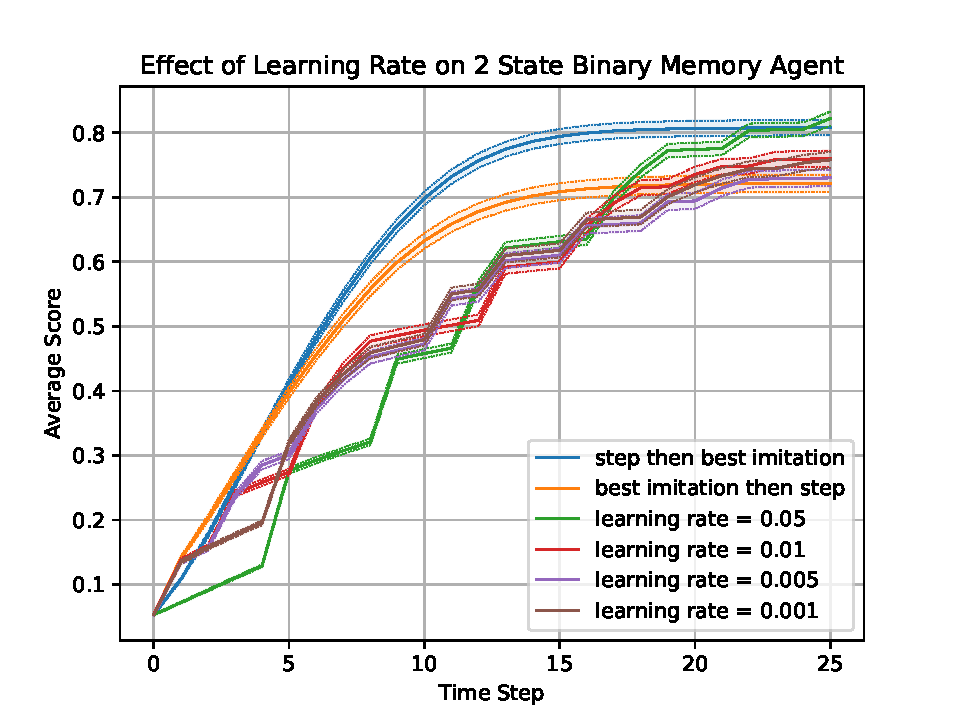
\includegraphics[width=16em]{../figures/comparison_b2.pdf}
        \caption{Memory Size of 2 bits}
        \label{comp_b2}
    \end{subfigure}
    \begin{subfigure}[b]{0.32\textwidth}
        \centering
        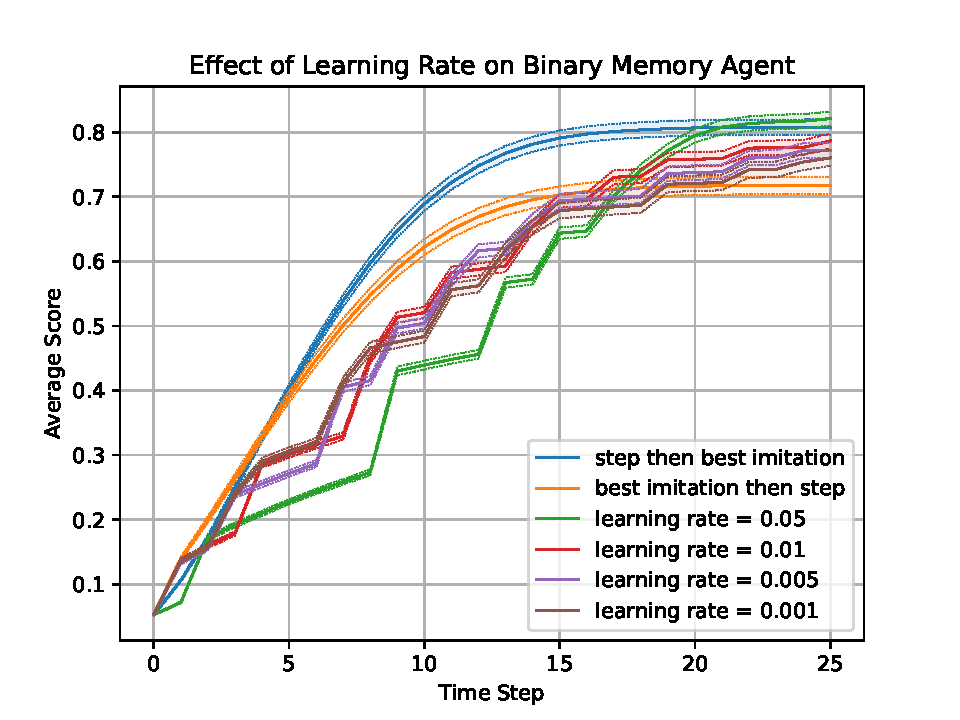
\includegraphics[width=16em]{../figures/comparison_b3.pdf}
        \caption{Memory Size of 3 bits}
        \label{comp_b3}
    \end{subfigure}
    \begin{subfigure}[b]{0.32\textwidth}
        \centering
        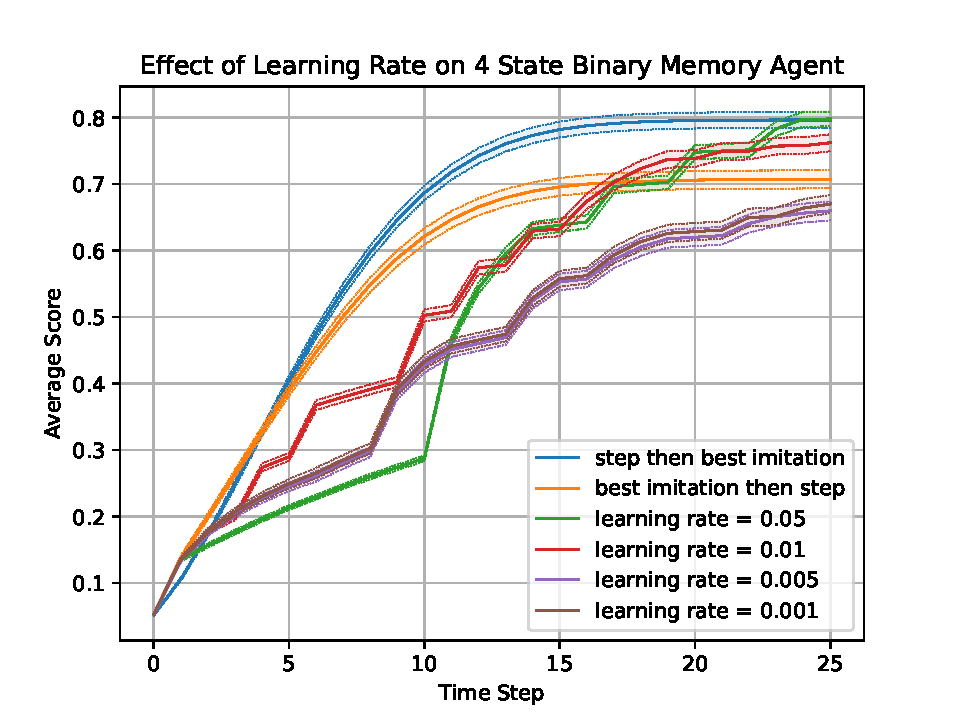
\includegraphics[width=16em]{../figures/comparison_b4.pdf}
        \caption{Memory Size of 4 bits}
        \label{comp_b4}
    \end{subfigure}
    \caption{
        The Average and 95\% confidence of the Average Node Score
        at each time step.
    }
    \label{comp}
\end{figure}

\begin{figure}[ht]
    \centering
    \begin{subfigure}[b]{0.24\textwidth}
        \centering
        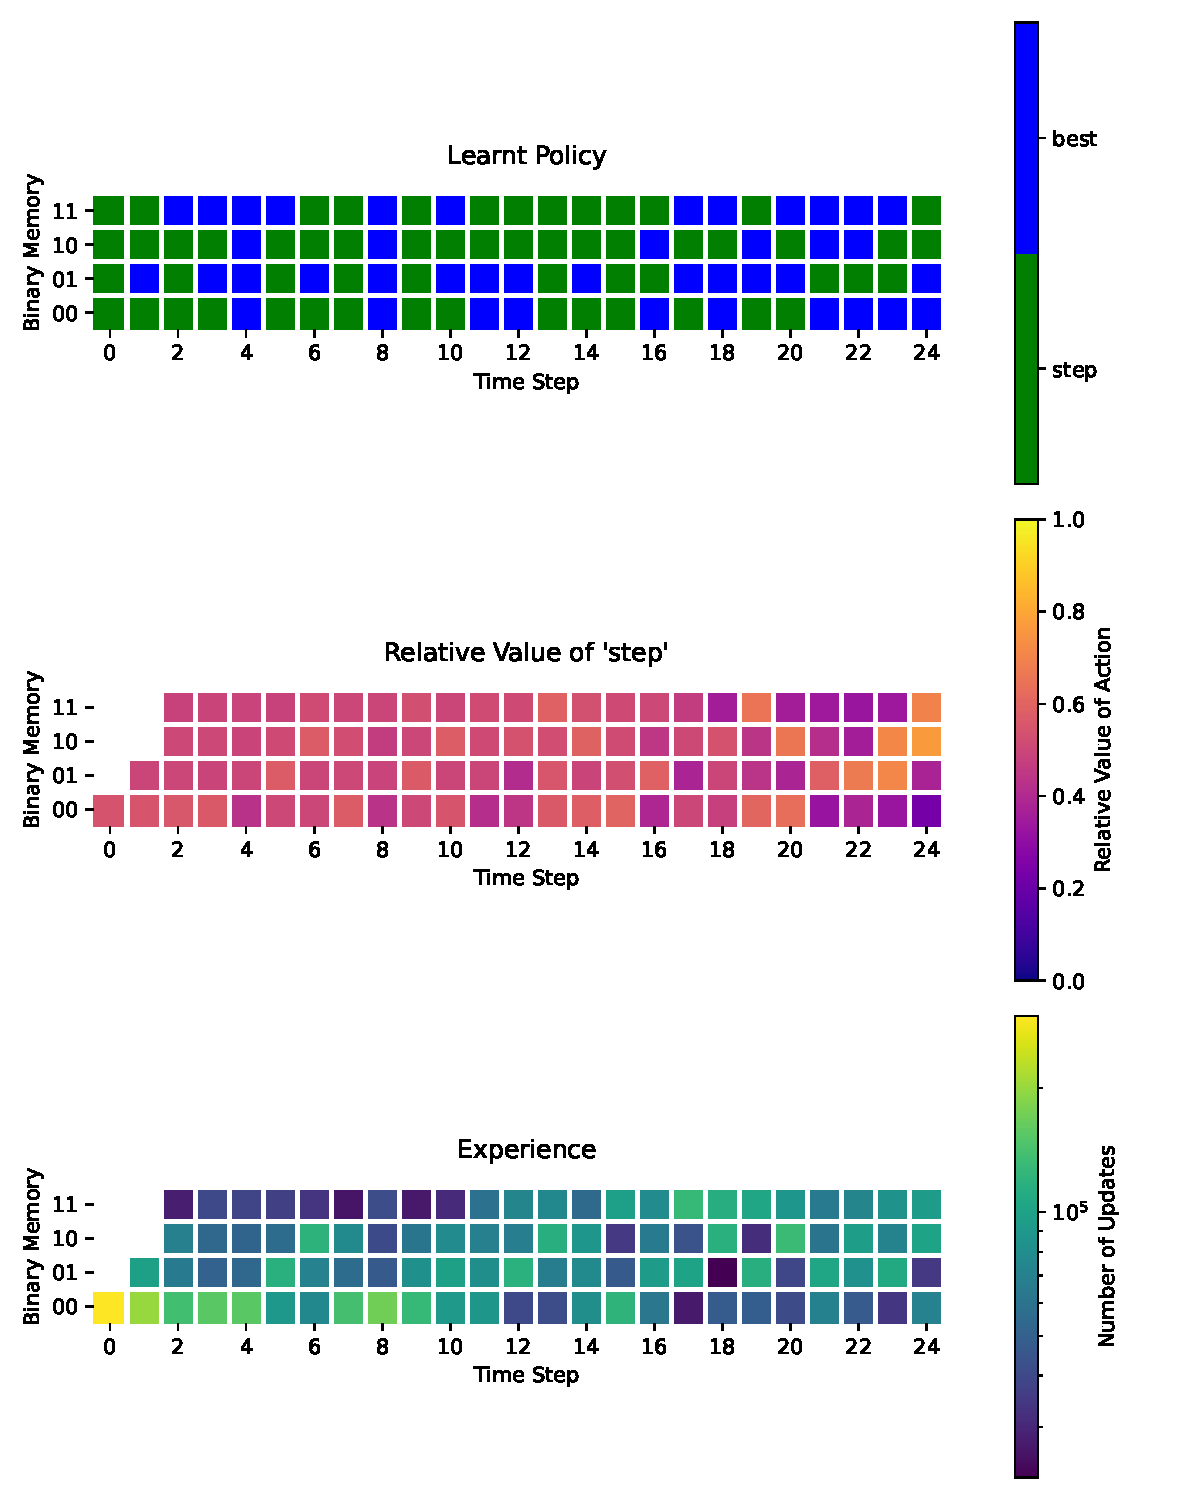
\includegraphics[width=12em]{../figures/policy_b2_lr05.pdf}
        \caption{Learning Rate of 0.05}
        \label{b2_lr05}
    \end{subfigure}
    \begin{subfigure}[b]{0.24\textwidth}
        \centering
        
\includegraphics[width=12em]{../figures/policy_b2_lr01.pdf}
        \caption{Learning Rate of 0.01}
        \label{b2_lr01}
    \end{subfigure}
    \begin{subfigure}[b]{0.24\textwidth}
        \centering
        
\includegraphics[width=12em]{../figures/policy_b2_lr005.pdf}
        \caption{Learning Rate of 0.005}
        \label{b2_lr005}
    \end{subfigure}
    \begin{subfigure}[b]{0.24\textwidth}
        \centering
        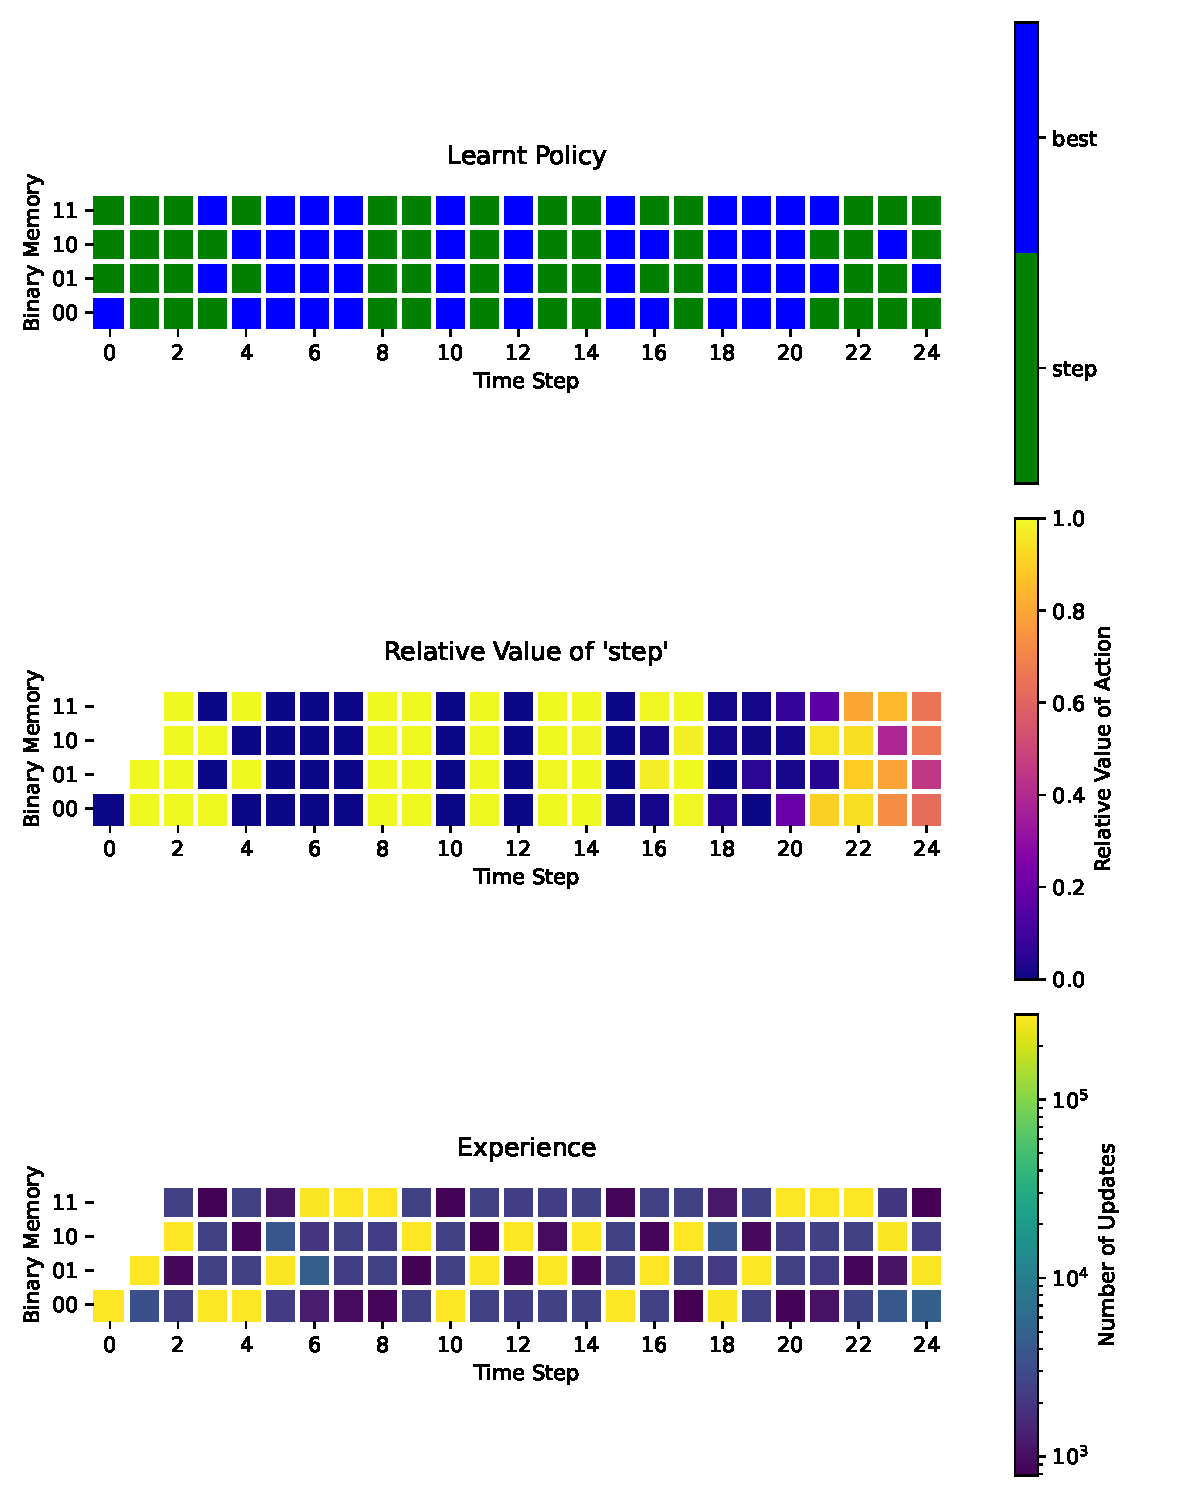
\includegraphics[width=12em]{../figures/policy_b2_lr001.pdf}
        \caption{Learning Rate of 0.001}
        \label{b2_lr001}
    \end{subfigure}
    \caption{
        The policy, experiance, and relative value of the action `step'
        over best for a binary agents with a memory size of two bits
        and varying learning rates. The most recent timestep
        is the least significant bit of the memory.
        The action `best' is represented by a `1' and `step' by a `0'.
    }
    \label{policy_b2}
\end{figure}


\begin{figure}[ht]
    \centering
    \begin{subfigure}[b]{0.24\textwidth}
        \centering
        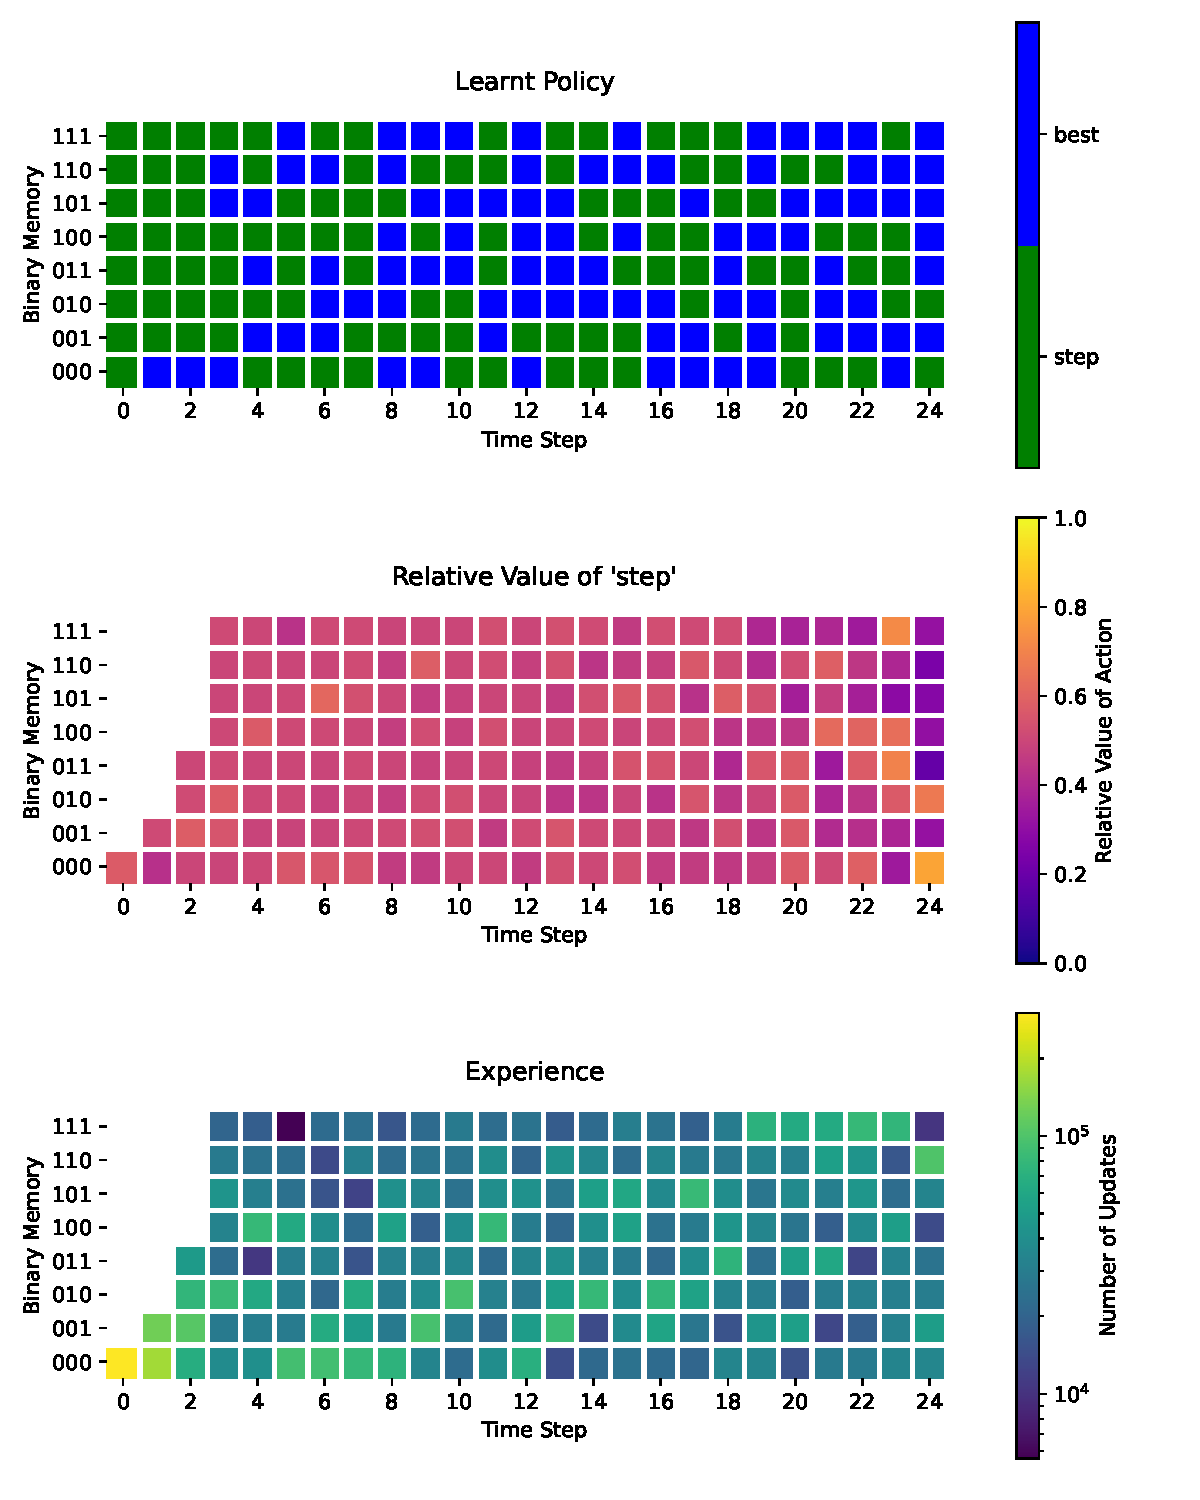
\includegraphics[width=12em]{../figures/policy_b3_lr05.pdf}
        \caption{Learning Rate of 0.05}
        \label{b3_lr05}
    \end{subfigure}
    \begin{subfigure}[b]{0.24\textwidth}
        \centering
        
\includegraphics[width=12em]{../figures/policy_b3_lr01.pdf}
        \caption{Learning Rate of 0.01}
        \label{b3_lr01}
    \end{subfigure}
    \begin{subfigure}[b]{0.24\textwidth}
        \centering
        
\includegraphics[width=12em]{../figures/policy_b3_lr005.pdf}
        \caption{Learning Rate of 0.005}
        \label{b3_lr005}
    \end{subfigure}
    \begin{subfigure}[b]{0.24\textwidth}
        \centering
        
\includegraphics[width=12em]{../figures/policy_b3_lr001.pdf}
        \caption{Learning Rate of 0.001}
        \label{b3_lr001}
    \end{subfigure}
    \caption{
        The policy, experiance, and relative value of the action `step'
        over best for a binary agents with a memory size of three bits
        and varying learning rates. The most recent timestep
        is the least significant bit of the memory.
        The action `best' is represented by a `1' and `step' by a `0'.
    }
    \label{policy_b3}
\end{figure}

\begin{figure}[ht]
    \centering
    \begin{subfigure}[b]{0.24\textwidth}
        \centering
        
\includegraphics[width=12em]{../figures/policy_b4_lr05.pdf}
        \caption{Learning Rate of 0.05}
        \label{b4_lr05}
    \end{subfigure}
    \begin{subfigure}[b]{0.24\textwidth}
        \centering
        
\includegraphics[width=12em]{../figures/policy_b4_lr01.pdf}
        \caption{Learning Rate of 0.01}
        \label{b4_lr01}
    \end{subfigure}
    \begin{subfigure}[b]{0.24\textwidth}
        \centering
        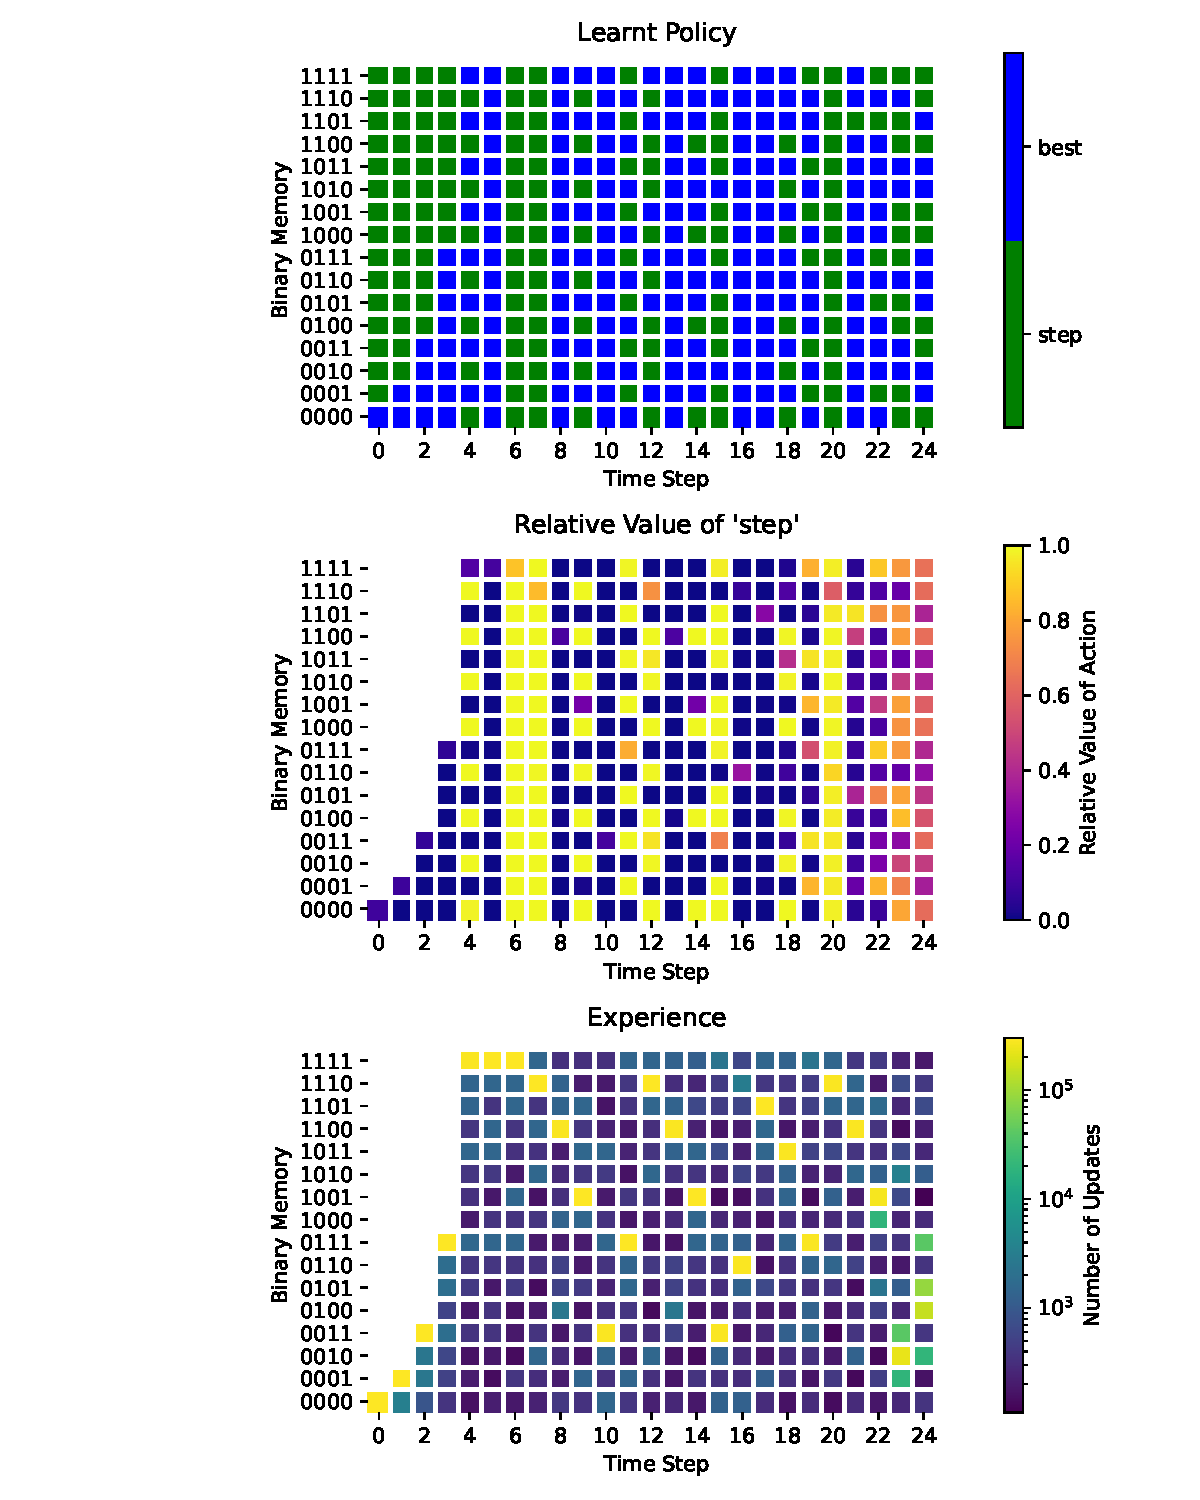
\includegraphics[width=12em]{../figures/policy_b4_lr005.pdf}
        \caption{Learning Rate of 0.005}
        \label{b4_lr005}
    \end{subfigure}
    \begin{subfigure}[b]{0.24\textwidth}
        \centering
        
\includegraphics[width=12em]{../figures/policy_b4_lr001.pdf}
        \caption{Learning Rate of 0.001}
        \label{b4_lr001}
    \end{subfigure}
    \caption{
        The policy, experiance, and relative value of the action `step'
        over best for a binary agents with a memory size of four bits
        and varying learning rates. The most recent timestep
        is the least significant bit of the memory.
        The action `best' is represented by a `1' and `step' by a `0'.
    }
    \label{policy_b4}
\end{figure}


\end{document}
